\chapter{Introduction}
Breast cancer affects 1 in 8 women in the United States. It is the second leading cause of cancer deaths amongst women. Mammography has shown to be beneficial for early detection of breast cancer \cite{Nystrom:2002hb}. Currently, the American Cancer Society recommends that women with no specific risk for breast cancer get yearly screening mammograms to catch potentially malignant findings early \cite{Smith:2003en}. The mammography report is of crucial importance, since it conveys the radiologist findings, interpretation of those findings in terms of likelihood of malignancy, and suggested patient management, such as follow-up imaging or biopsy. However, a major barrier to mammography for breast cancer detection and workup is the inherent qualitative nature of current mammography reporting practices which results in variation in practice and non-standard quality of patient care.

Substantial variability with regards to sensitivity and specificity of evaluation of lesion malignancy in mammograms has been shown amongst different readers as well as different facilities \cite{Jackson:2009fw, Beam:1996ui, Elmore:2002vc, Taplin:2008bv}. Moreover, it has been shown that variability occurs in the content of the report, with findings that are not consistent amongst readers and not complete with respect to the image content \cite{Hobby:2000th, Robinson:1997uq}. Prior studies have shown the importance of good reporting practices and identified several key traits of good reports: correctness of findings, completeness of the description of significant clinical findings, consistency of report language and findings, and timeliness of the report’s completion \cite{Johnson:2004kh, HaraldO:2004hi}. Hence, variability in the report directly hampers the utility of mammographic diagnosis. False positives and defensive medical decision making cause patient anxiety, excessive additional invasive testing (e.g., biopsy), and rising healthcare costs, while false negatives result in delayed treatment at the expense of patient health.

Efforts to improve upon consistency and clarity of report language include the Breast Imaging-Reporting and Data System (BIRADS) which provides a standard lexicon of descriptors for radiological observations \cite{Liberman:ws}. Additionally, Structured Reporting Systems have been designed to improve the quality of radiology reporting by providing templates with standardized information and support for BIRADS \cite{Reiner:2009ib}. Unfortunately, structured reporting is generally more time-intensive and imposes distractions in the traditional radiological workflow, directly interfering with timeliness \cite{Weiss:2008er}. Moreover, these two approaches mainly aim to improve upon reporting language and clarity, not analyze report content. To this effect, Decision Support Systems (DSS) have been developed to improve upon mammography interpretation and diagnosis \cite{Garg:2005cb, Burnside:2000wl, ElizabethS:2005gc, Rubin:2005jg}. DSS are tools that incorporate medical information to provide meaningful input to medical practitioners. However, to date, adoption of DSS has limited as they often interrupt the radiological workflow \cite{Morgan:2011ct}. In addition, decision support has only focused on diagnosis and automated computational analysis of image data. There has been little work using DSS to improve consistency and completeness of mammographic reporting, which ultimately would be important for improving radiologist diagnostic accuracy in assessing lesions on mammography. Our hypothesis is that improving the consistency and completeness in mammography reporting can improve the sensitivity and specificity of cancer diagnosis and thereby improve the quality of patient care.

To tackle this challenge and to enable translation of DSS into clinical practice to benefit patient care, we propose a real-time DSS that provides feedback to radiologists as they generate their reports. This system will create a structured radiological report that is verified for consistency and completeness. This differs from traditional approaches to DSS because our system will improve reporting practice. By ensuring that the relevant observations are consistently and completely described in mammography reports, our DSS will reduce variability in practice, improving practitioner decision making and lead to better patient care.

\section{FASR: Fast Adaptive Structured Reporting}
The Fast Adaptive Structured Reporting (FASR) system's goal is to reduce variability and error in radiological interpretation by providing decision-support during reporting time. This works by incorporating multiple checks during the reporting process and providing real-time feedback to the radiologist.

There are three main components to FASR: (1) Verification of the annotation correctness, (2) verification of reporting completeness and (3) providing feedback to the radiologist. In this chapter, we will explain in-depth how FASR solves these tasks.

\begin{figure}[h]
	\centering
	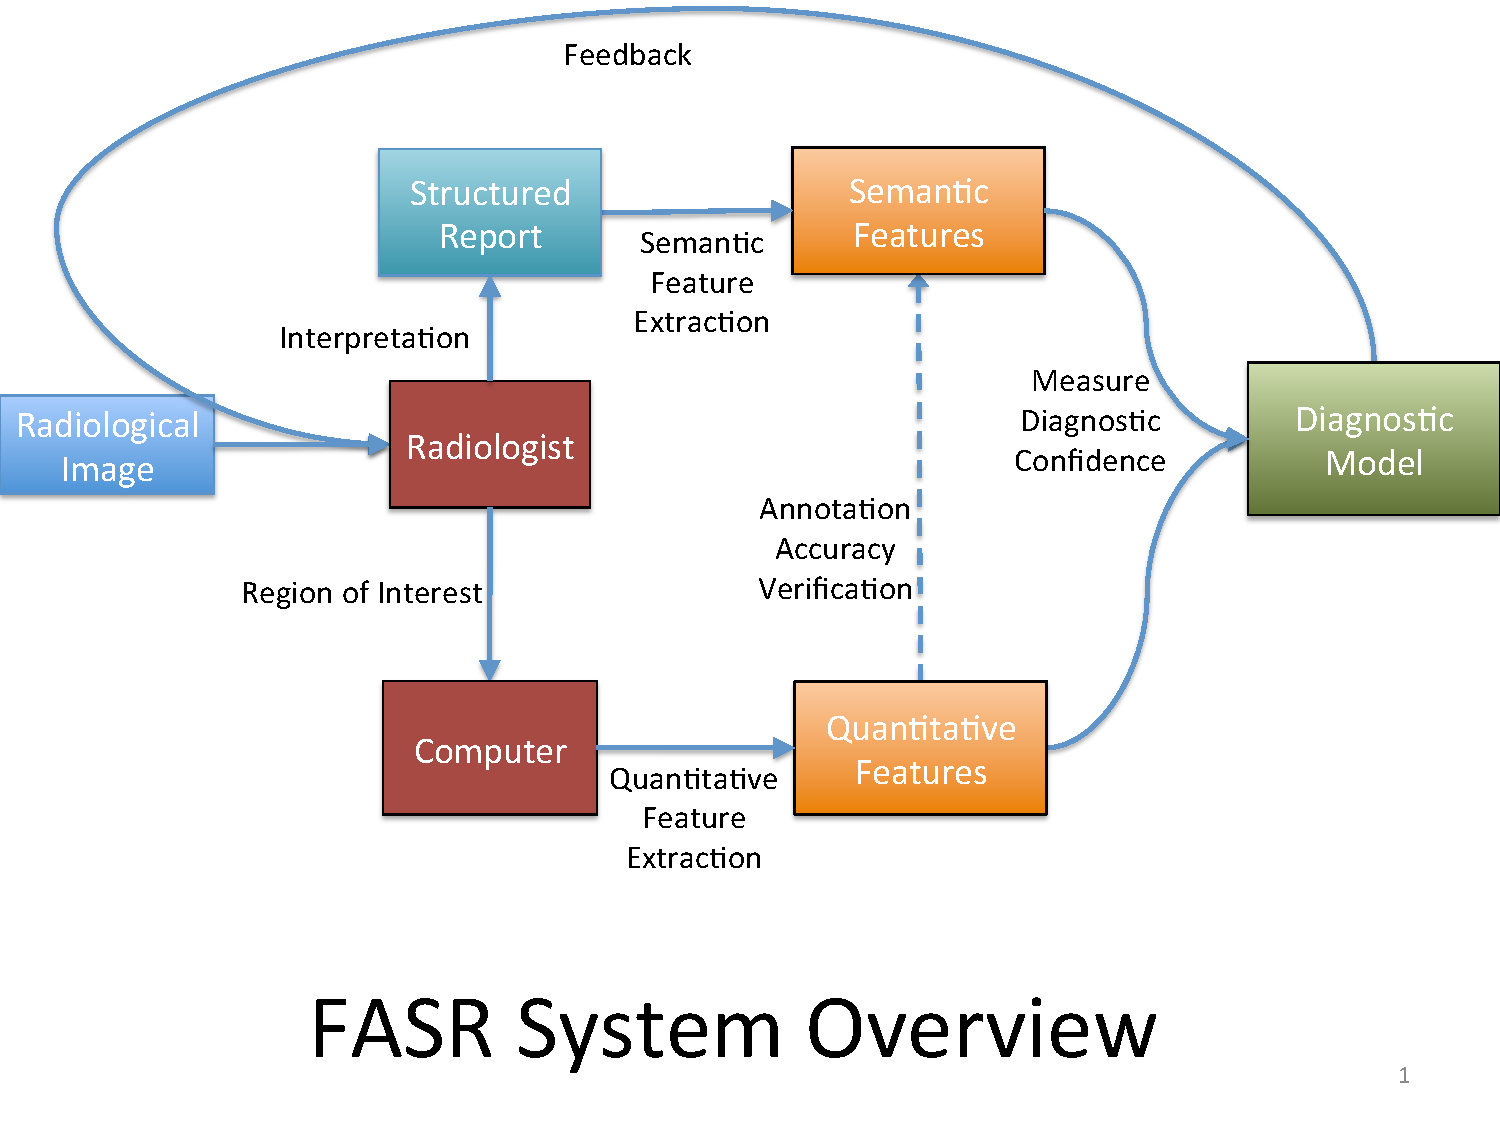
\includegraphics[width=1\linewidth]{fasr_diagram.pdf}
	\caption{Overview of the Fast Adaptive Structured Reporting (FASR) system}
	\label{fig:fasr_diagram}
\end{figure}
